\section{Introduzione}
	
	\begin{frame}
		\frametitle{Presentazione dei dati}	
		\begin{block}{Dataset}
			\begin{itemize}
				\item 721 \torange{osservazioni} riguardanti i \pok delle prime sei generazioni
				\item 23 \torange{variabili} che descrivono le loro caratteristiche fisiche e di combattimento
			\end{itemize}
		\end{block}					
		\begin{center}
			\begin{figure}
				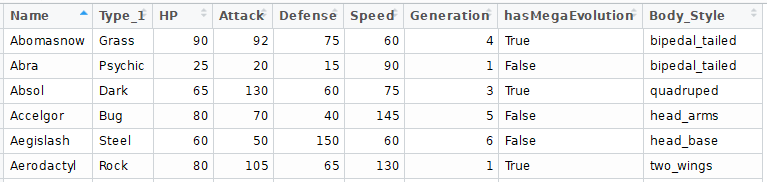
\includegraphics[width=\textwidth]{img/screenDati}
			\end{figure}
		\end{center}
	\end{frame}

\section{Analisi descrittiva}

	\begin{frame}
		\frametitle{Analisi descrittiva}
		\begin{block}{Pulizia dataset}
			\begin{itemize}
				\item Rimozione delle colonne non necessarie (ID, Nome, ecc.)
				\item Rimozione degli eventuali NA 
			\end{itemize}
		\end{block}
		\begin{block}{Preparazione categorie}
			\begin{itemize}
				\item \torange{Attack} è una variabile intera che va da 5 a 165
				\item La trasformiamo in \torange{categorica} su 4 livelli
				\begin{itemize}
					\item \torange{Low} (5:45)
					\item \torange{Med-Low} (46:85)
					\item \torange{Med-Hig} (86:125)
					\item \torange{High} (126:165)
				\end{itemize}
			\end{itemize}
		\end{block}
	\end{frame}

	\begin{frame}
		\begin{block}{Creazione grafici}
			\begin{itemize}
				\item Raggruppamento per categoria delle altre variabili significative
				\item Calcolo della media
				\item Costruzione dei grafici
			\end{itemize}
		\end{block}
		\begin{columns}
			\begin{column}{0.45\textwidth}
				\begin{center}
					\begin{figure}
						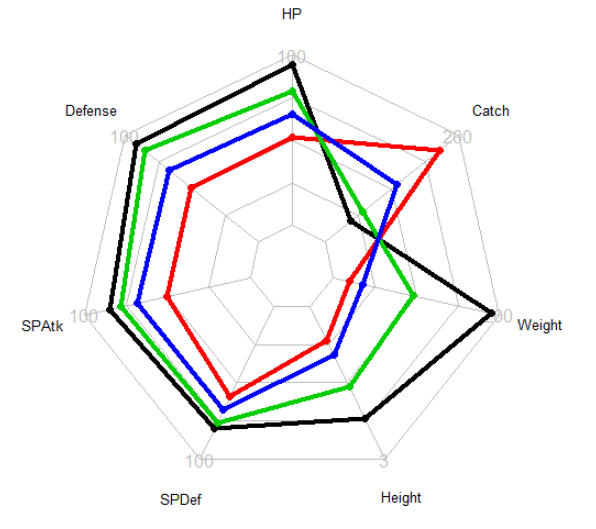
\includegraphics[width=\columnwidth]{img/radar}
						\caption{Radarchart}
					\end{figure}
				\end{center}
			\end{column}
			\begin{column}{0.55\textwidth}
				\begin{center}
					\begin{figure}
						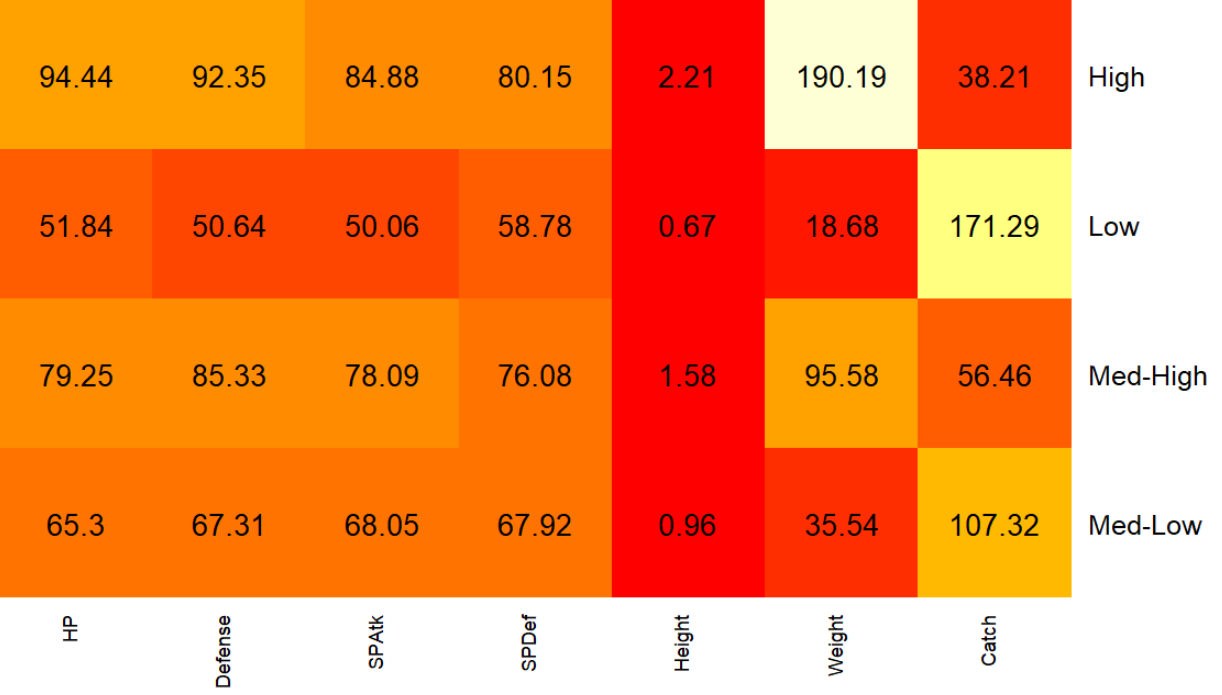
\includegraphics[width=\columnwidth]{img/heat}
						\caption{Heatmap}
					\end{figure}
				\end{center}
			\end{column}
		\end{columns}
	\end{frame}

\section{CART}

	\begin{frame}
		\frametitle{CART}
		\begin{block}{Definizioni}
			\begin{itemize}
				\item Usiamo i CART per dedurre il valore delle grandezze non note a partire da informazioni conosciute
				\item \textbf{Classification trees}: partizionamento ricorsivo dello spazio dei predittori, nel quale ad ogni elemento viene assegnata una classe di predizione
				\item Ad ogni ramo (\torange{nodo padre}) si applica una separazione binaria dei dati (\torange{split}), così da ottenere altri rami (\torange{nodi figli}) fino ai nodi terminali (\torange{foglie})
			\end{itemize}
		\end{block}
	\end{frame}

	\begin{frame}
		\frametitle{Costruzione Tree}
		{\footnotesize
		\begin{block}{Valutazione degli split}
			\begin{itemize}
				\item Favorire \torange{omogeneità} dei nodi ed \torange{eterogeneità} dei nodi figli
				\item Lo scopo è \torange{minimizzare} l'impurezza dei nodi figli calcolata attraverso:
				\begin{itemize}
					\item Indice di \torange{Entropia} $= - \sum_{k=1}^{K} p_k * \log_2 (p_k)$
					\item Indice di \torange{Gini} $= \sum_{k=1}^{K}(p_k)(1-p_k)$
				\end{itemize}
				\item Impurezza = 0 $\Leftrightarrow$ il valore della variabile di risposta è lo stesso per tutte le osservazioni all'interno del nodo
			\end{itemize}
		\end{block}
		\begin{block}{Assegnazione delle categorie ai nodi}
			\begin{itemize}
				\item Ogni nodo è etichettato con una modalità della variabile di risposta
				\item Ogni etichetta viene assegnata minimizzando il classification error rate
				\item Nel caso sia uguale per tutte le modalità si sceglie quella più numerosa
			\end{itemize}
		\end{block}}
	\end{frame}

	\begin{frame}
		\frametitle{Costruzione Tree}
		{\footnotesize
		\begin{block}{Criteri di arresto}
			\begin{itemize}
				\item Numero di osservazioni minimo per ogni nodo
				\item Purezza dei nodi maggiore di un valore fissato
				\item Profondità dell'albero limitata
				\item Valori identici per tutti i predittori
			\end{itemize}
		\end{block}
		\begin{block}{Potatura}
			\begin{itemize}
				\item Facciamo crescere totalmente l'albero per poi potarlo successivamente
				\item Utilizziamo metodi per individuare il numero di rami che ci garantiscano il minore classification error rate
				e la minima complessità dell'albero
				\item Ad esempio \torange{K-fold cross validation}
			\end{itemize}
		\end{block}}
	\end{frame}

	\begin{frame}
		\frametitle{Validation}
		\begin{block}{K-fold cross validation}
			\begin{itemize}
				\item Dividiamo le osservazioni in K gruppi di simili dimensioni
				\item Usiamo un gruppo come \torange{validation set} e stimiamo sui rimanenti
				\item Ripetiamo la procedura K volte cambiando ogni volta il gruppo di validation set
				\item Scegliamo il valore che minimizza il \emph{cross validation error rate}
			\end{itemize}
		\end{block}
	\end{frame}

	\begin{frame}
		\frametitle{Trees}	
		\begin{center}
			\begin{figure}
				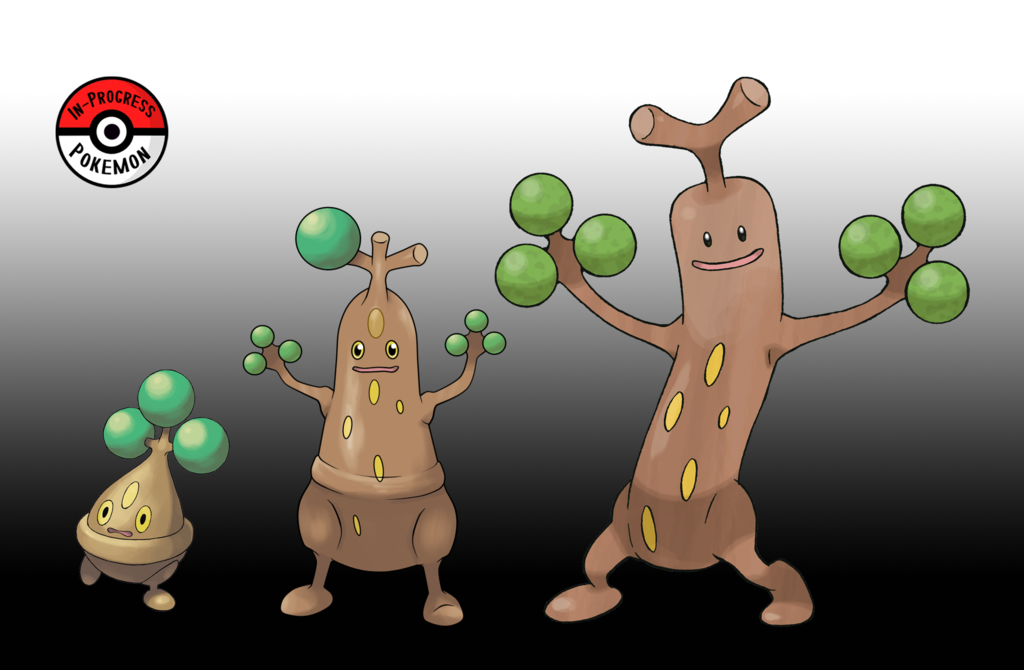
\includegraphics[width=0.94\textwidth]{img/pokpianta}
			\end{figure}
		\end{center}
	\end{frame}

	\begin{frame}
		\frametitle{Trees}	
		\begin{block}{Obiettivo}
			\begin{itemize}
				\item Predire quali \pok hanno un alto valore di attacco utilizzando
				\begin{itemize}
					\item \textbf{Classification trees} (\torange{Indice di Gini} e \torange{Indice di Entropia}) usando i pacchetti \emph{rpart} e \emph{tree}
					\item \textbf{Conditional inference trees} usando il pacchetto \emph{party}
					\item \textbf{Evolutionary learning of globally optimal trees} usando il pacchetto \emph{evtree}
				\end{itemize}
				\item Confrontare i risultati ottenuti
			\end{itemize}
		\end{block}		
	\end{frame}

	\begin{frame}
		\frametitle{Trees}	
		\begin{block}{Variabile di risposta}
			\begin{itemize}
				\item Siamo interessati ai \pok con valore di attacco \emph{High}. Aggiungiamo la relativa variabile di risposta al dataset
				\item Dividiamo in maniera casuale le osservazioni in due insiemi, uno di \torange{training} e uno di \torange{testing}
			\end{itemize}
		\end{block}
		\begin{center}
			\begin{figure}
				\lstinputlisting[firstline=72, lastline=79]{code/pokfine.R}
			\end{figure}
		\end{center}
	\end{frame}

	\begin{frame}
		\frametitle{Pacchetto RPART}
		\begin{block}{Caratteristiche principali}
			\begin{itemize}
				\item Il metodo di split di default utilizza l'indice di Gini. In alternativa permette l'utilizzo dell'indice di Entropia.
				\item La dimensione minima di ogni nodo deve essere 20
				\item La profondità massima dell'albero è 30
			\end{itemize}
		\end{block}
	\end{frame}


	\begin{frame}
		\frametitle{Pacchetto RPART}
		\begin{center}
			\begin{figure}
				\lstinputlisting[basicstyle=\tiny, firstline=150, lastline=152]{code/pokfine.R}
			\end{figure}
			\begin{figure}
				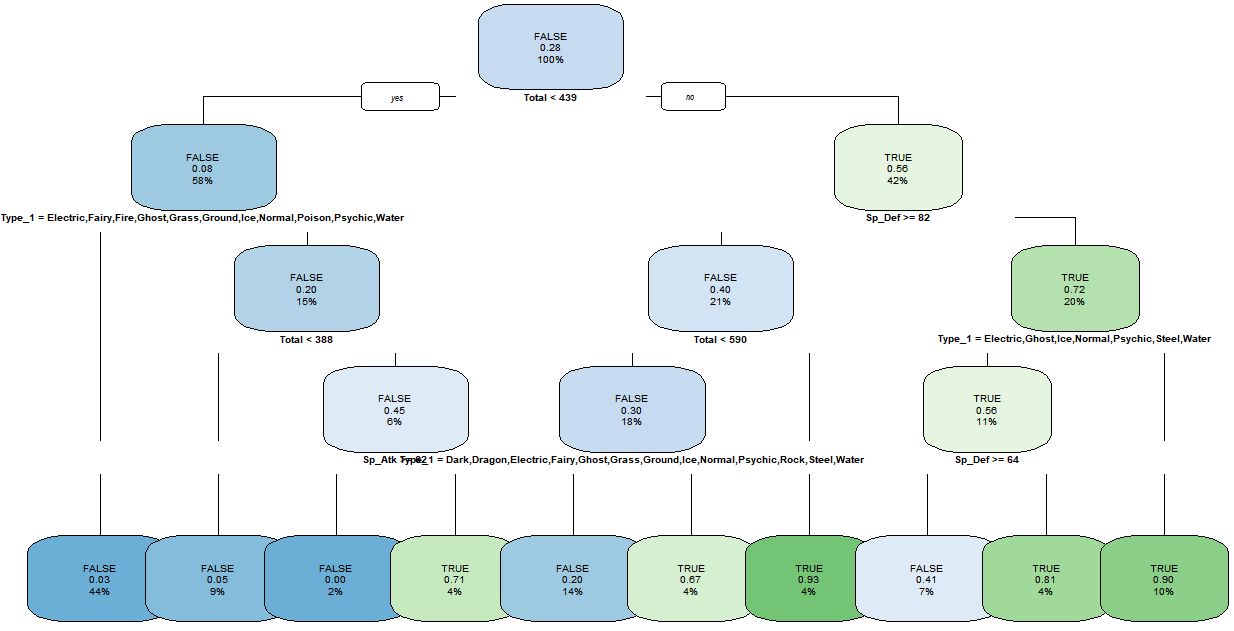
\includegraphics[width=0.94\textwidth]{img/rpartGini}
			\end{figure}
		\end{center}
	\end{frame}

	\begin{frame}
		\frametitle{Pacchetto RPART}
		\begin{center}
			\begin{figure}
				\lstinputlisting[firstline=158, lastline=159]{code/pokfine.R}
			\end{figure}
			\begin{figure}
				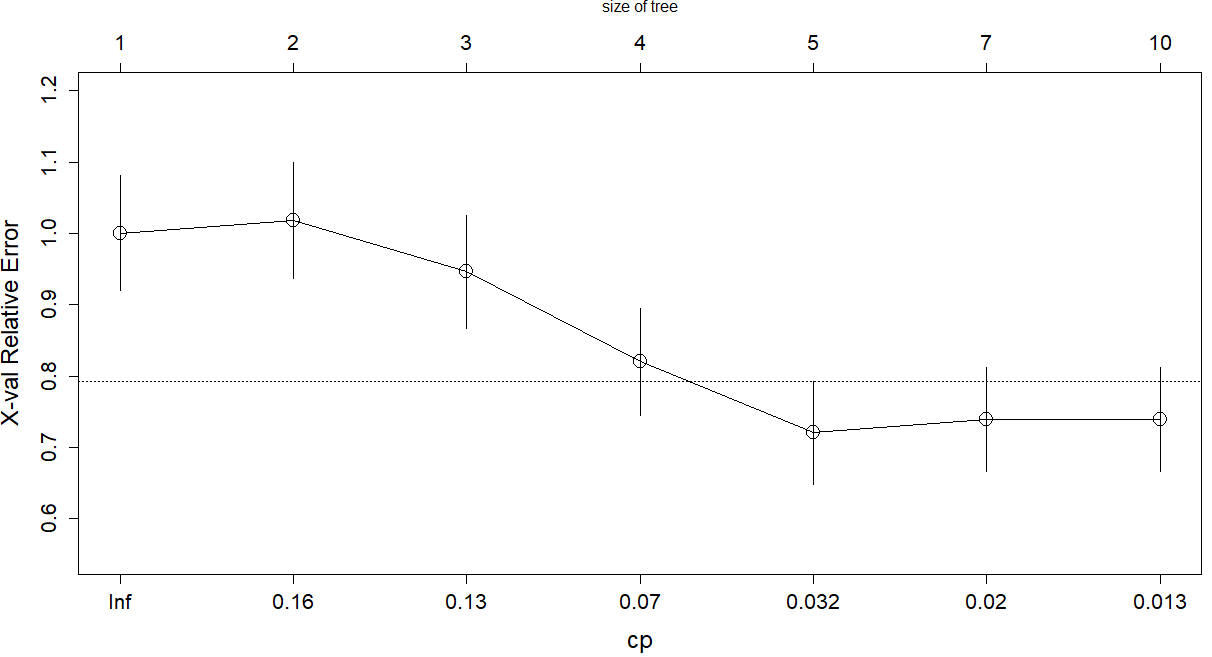
\includegraphics[scale=0.3]{img/cvginirpart}
			\end{figure}
		\end{center}
	\end{frame}


	\begin{frame}
		\frametitle{Pacchetto RPART}
		\begin{center}
			\begin{figure}
				\lstinputlisting[basicstyle=\tiny, firstline=160, lastline=162]{code/pokfine.R}
			\end{figure}
			\begin{figure}
				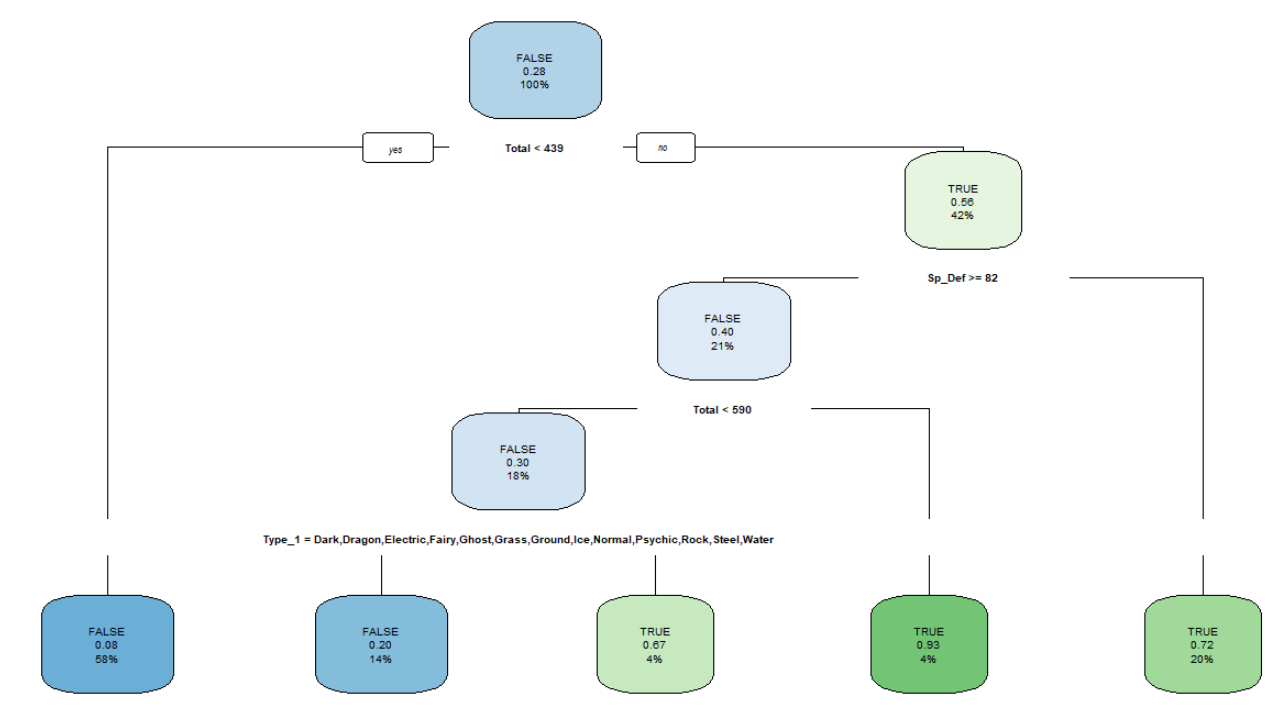
\includegraphics[scale=0.3]{img/rpartGinipr}
			\end{figure}
		\end{center}
	\end{frame}


	\begin{frame}
		\frametitle{Pacchetto RPART}
		\begin{center}
			\begin{figure}
				\lstinputlisting[basicstyle=\tiny, firstline=168, lastline=170]{code/pokfine.R}
			\end{figure}
			\begin{figure}
				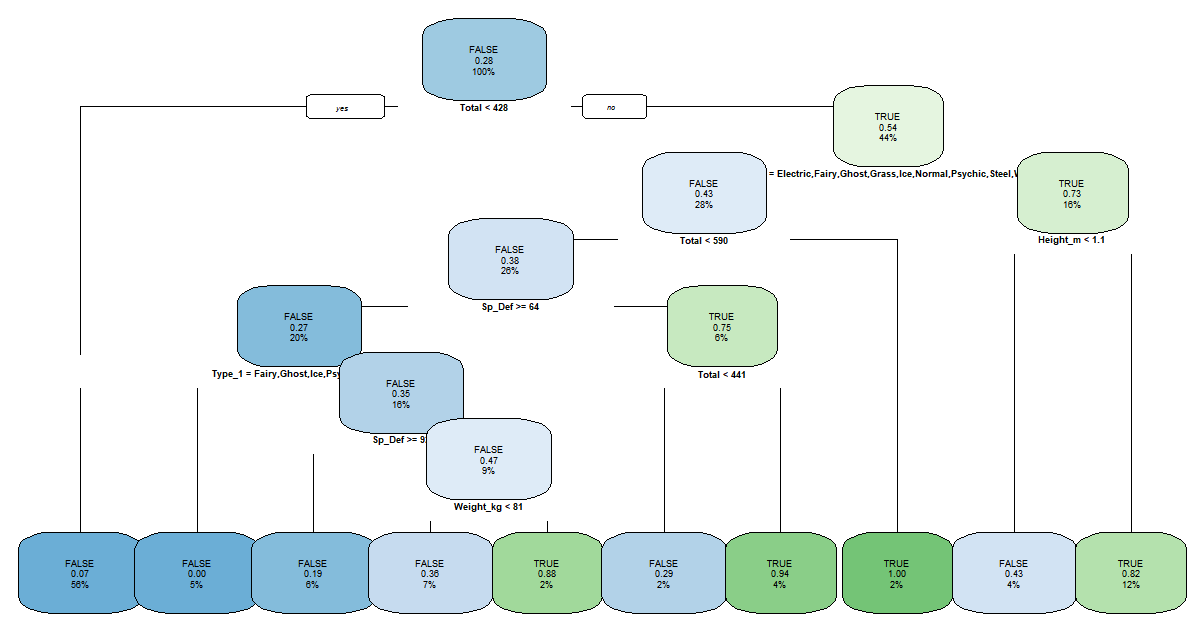
\includegraphics[width=0.9\textwidth]{img/rpartEntr}
			\end{figure}
		\end{center}
	\end{frame}

	\begin{frame}
		\frametitle{Pacchetto RPART}
		\begin{center}
			\begin{figure}
				\lstinputlisting[firstline=176, lastline=177]{code/pokfine.R}
			\end{figure}
			\begin{figure}
				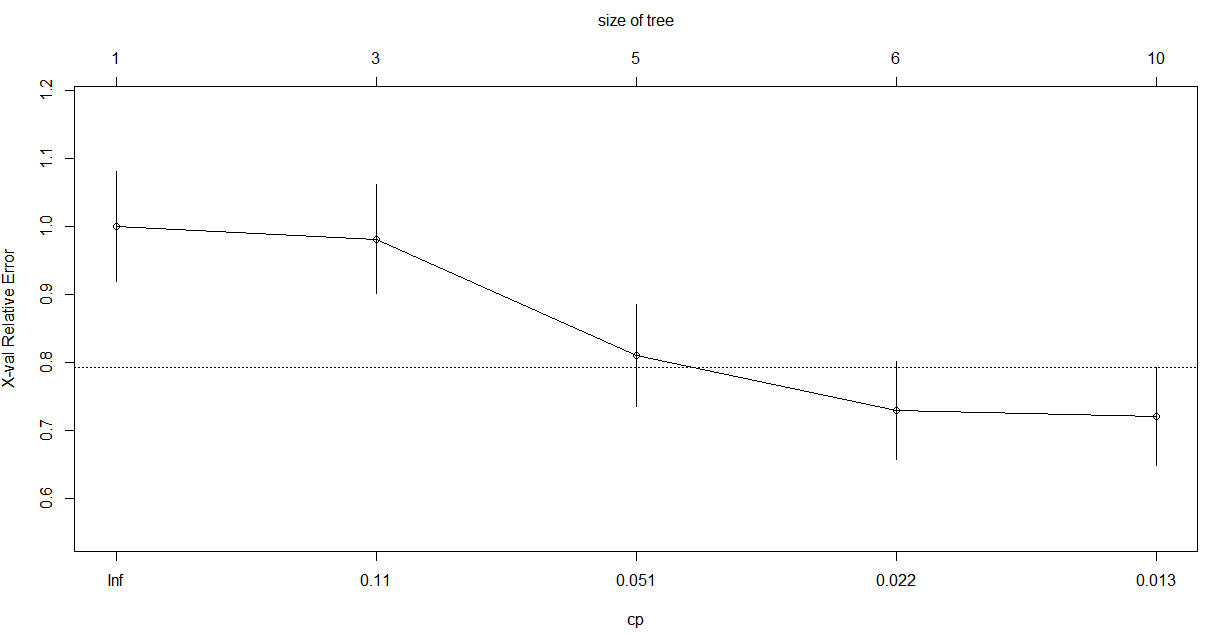
\includegraphics[scale=0.3]{img/cventrrpart}
			\end{figure}
		\end{center}
	\end{frame}

	\begin{frame}
		\frametitle{Pacchetto RPART}
		\begin{center}
			\begin{figure}
				\lstinputlisting[firstline=178, lastline=180]{code/pokfine.R}
			\end{figure}
			\begin{figure}
				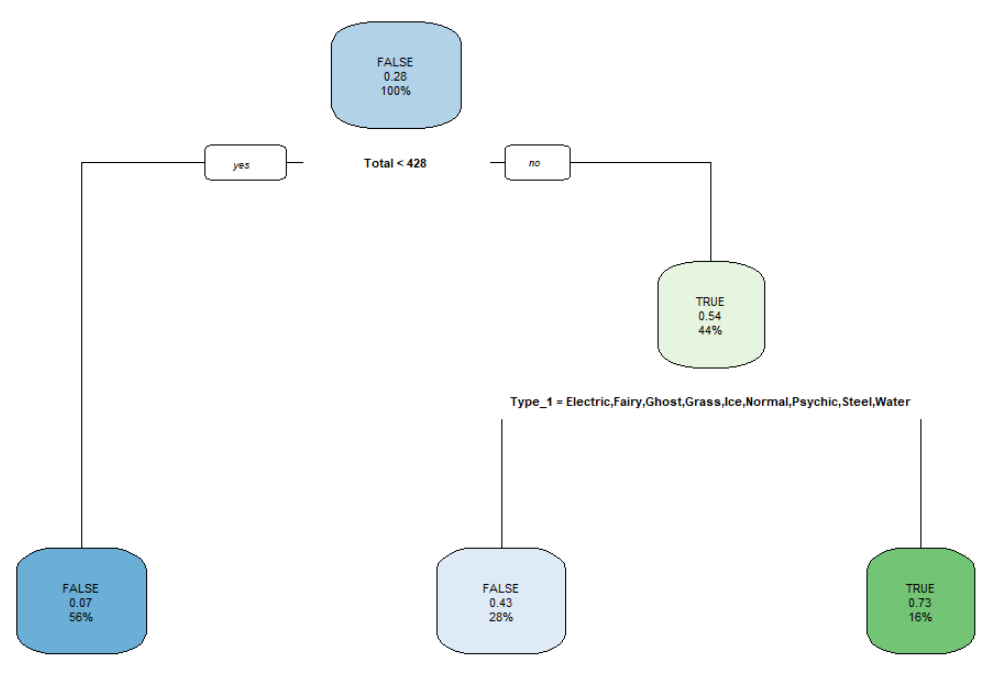
\includegraphics[scale=0.3]{img/rpartEntrpr}
			\end{figure}
		\end{center}
	\end{frame}


	\begin{frame}
		\frametitle{Pacchetto TREE}
		\begin{block}{Caratteristiche principali}
			\begin{itemize}
				\item Il metodo di split di default utilizza l'indice di Entropia. In alternativa permette l'utilizzo dell'indice di Gini.
				\item La dimensione minima di ogni nodo deve essere 10
				\item Lo split successivo avverrà se i figli conterranno almeno 5 osservazioni	
				\item La potatura avviene scegliendo la dimensione finale dell'albero che minimizza il cross validation error
			\end{itemize}
		\end{block}
	\end{frame}

	\begin{frame}
	\frametitle{Pacchetto TREE}
		\begin{center}
			\begin{figure}
				\lstinputlisting[basicstyle=\tiny, firstline=84, lastline=87]{code/pokfine.R}
			\end{figure}
			\begin{figure}
				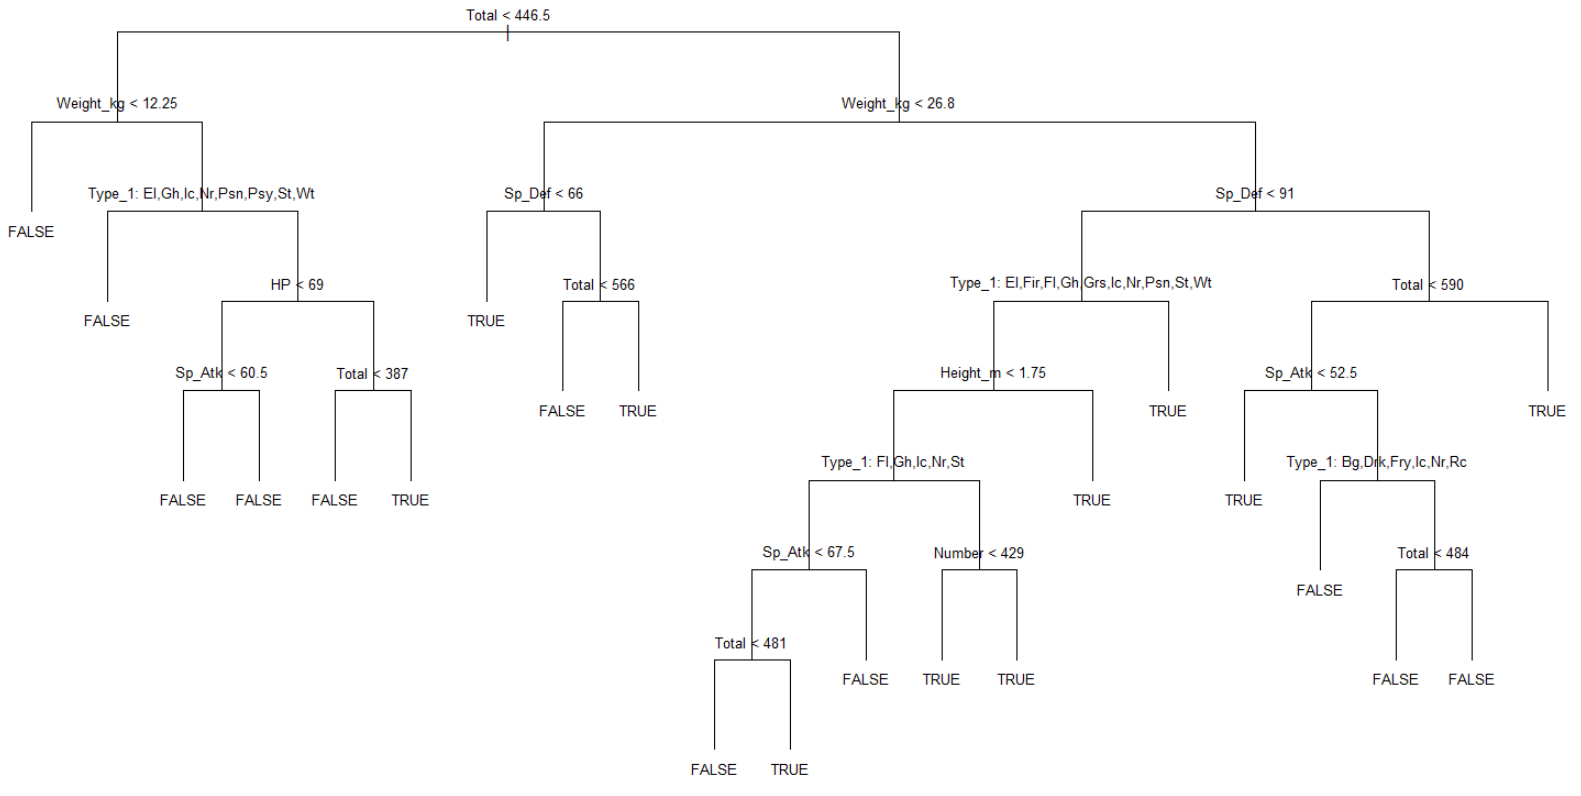
\includegraphics[width=0.95\textwidth]{img/treeEntr}
			\end{figure}
		\end{center}
	\end{frame}


	\begin{frame}
	\frametitle{Pacchetto TREE}
		\begin{center}
			\begin{figure}
				\lstinputlisting[firstline=101, lastline=103]{code/pokfine.R}
			\end{figure}
			\begin{columns}
				\begin{column}{0.5\textwidth}
					\begin{center}
						\begin{figure}
							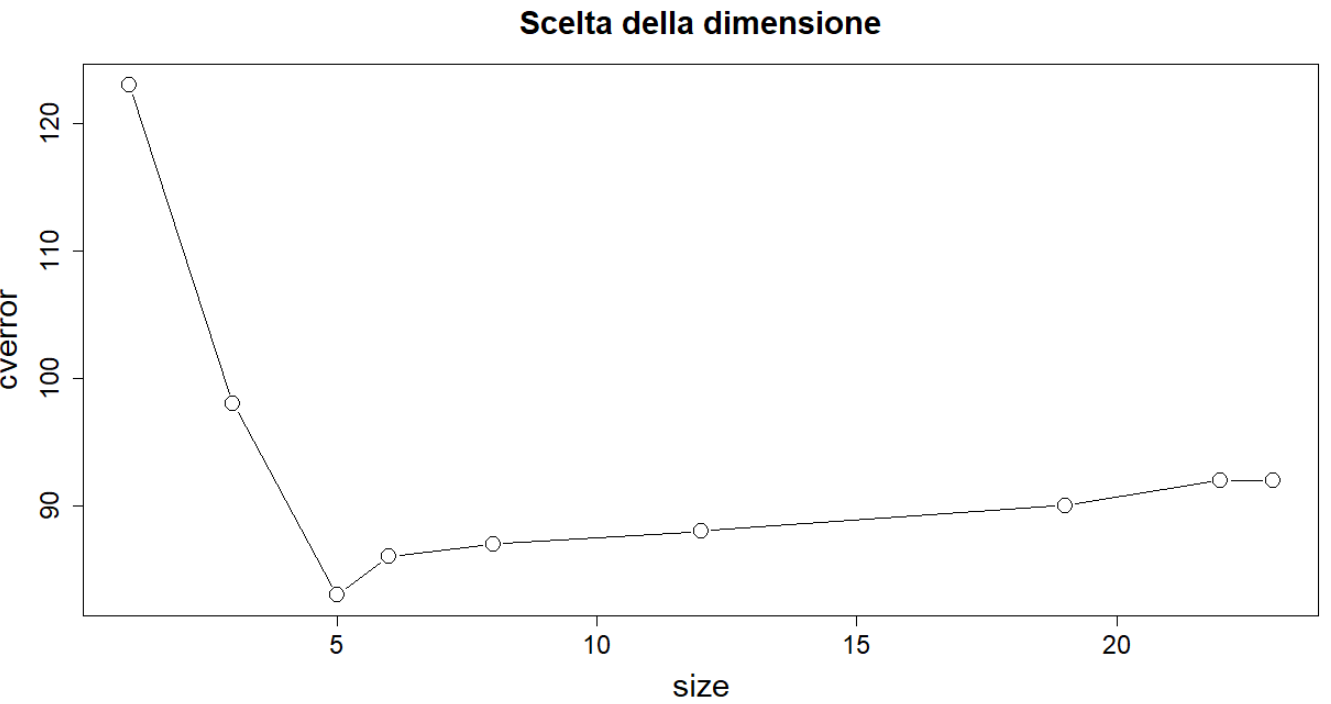
\includegraphics[width=\columnwidth]{img/cvdevtree}
						\end{figure}
						\begin{figure}
							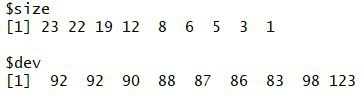
\includegraphics[width=\columnwidth]{img/cverrortree}
						\end{figure}
					\end{center}				
				\end{column}
				\begin{column}{0.5\textwidth}
					\begin{figure}
						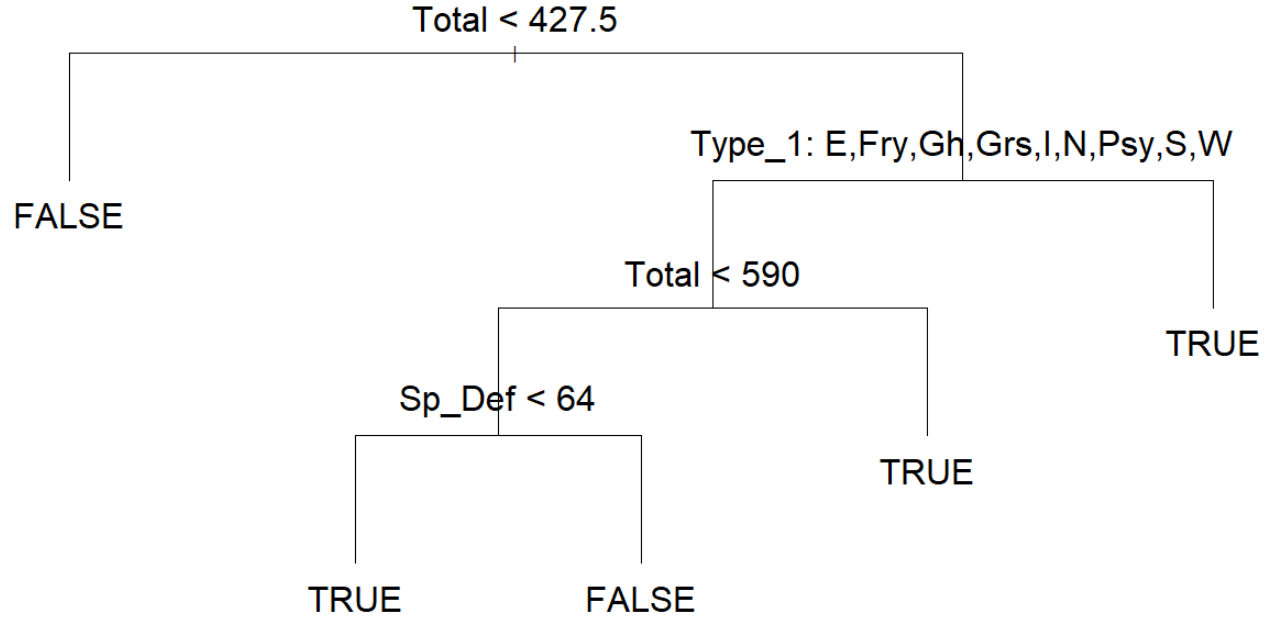
\includegraphics[width=\columnwidth]{img/treeEntrpr}
					\end{figure}
				\end{column}
			\end{columns}		
		\end{center}
	\end{frame}


	\begin{frame}
	\frametitle{Pacchetto TREE}
		\begin{center}
			\begin{figure}
				\lstinputlisting[basicstyle=\tiny, firstline=110, lastline=114]{code/pokfine.R}
			\end{figure}
			\begin{figure}
				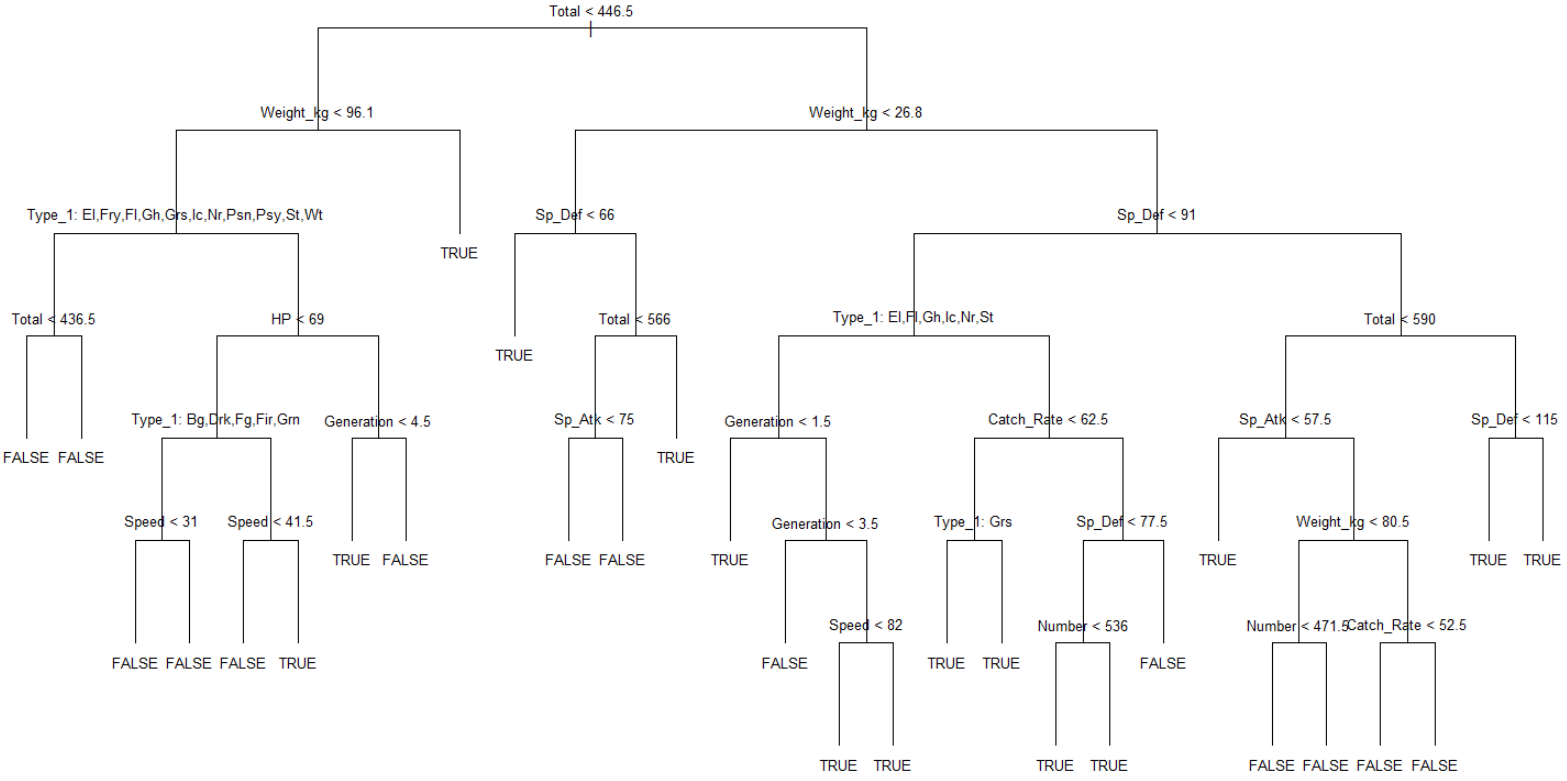
\includegraphics[width=0.95\textwidth]{img/treeGini}
			\end{figure}
		\end{center}
	\end{frame}

	\begin{frame}
	\frametitle{Pacchetto TREE}
		\begin{center}
			\begin{figure}
				\lstinputlisting[basicstyle=\tiny, firstline=126, lastline=128]{code/pokfine.R}
			\end{figure}
			\begin{columns}
				\begin{column}{0.5\textwidth}
					\begin{center}
						\begin{figure}
							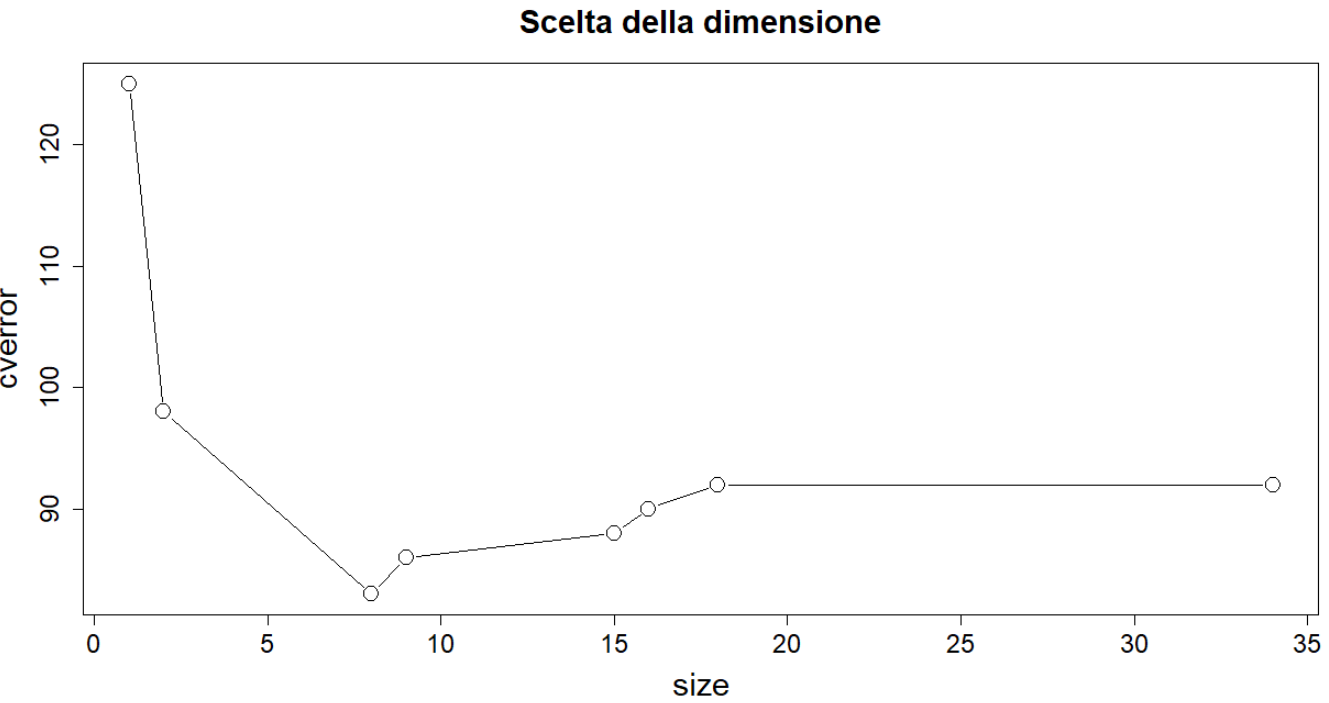
\includegraphics[width=\columnwidth]{img/cvginitree}
						\end{figure}
					\end{center}				
				\end{column}
				\begin{column}{0.5\textwidth}
					\begin{figure}
						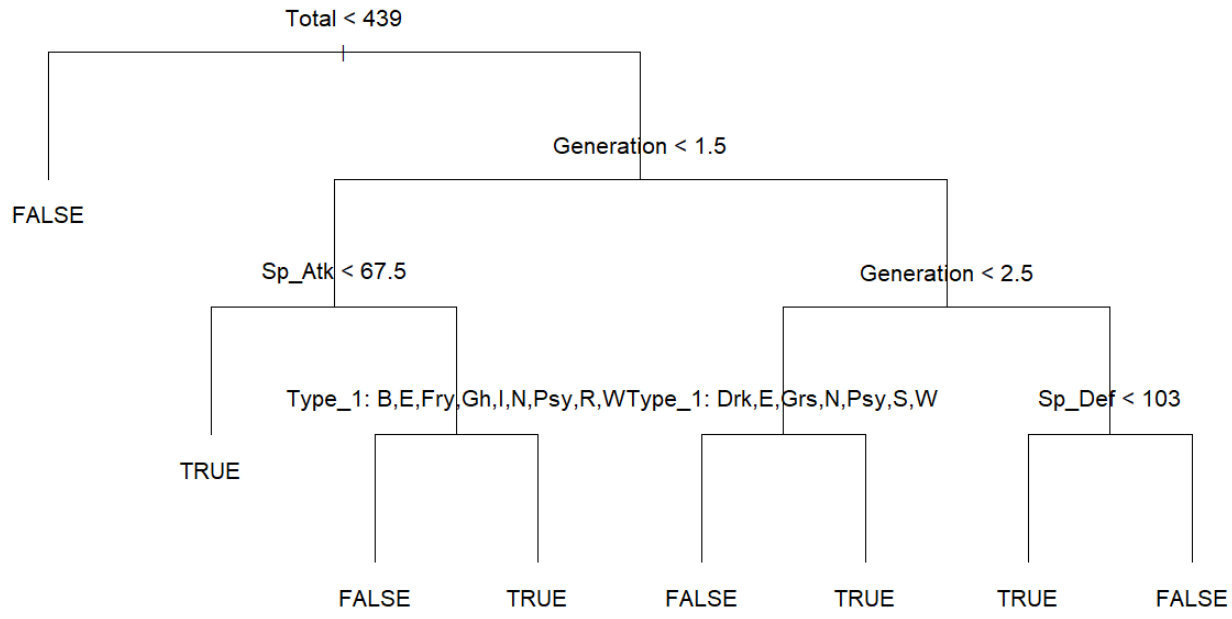
\includegraphics[width=\columnwidth]{img/treeGinipr2}
					\end{figure}
				\end{column}
			\end{columns}		
		\end{center}
	\end{frame}

	\begin{frame}
		\frametitle{Pacchetto PARTY}
		\begin{block}{Caratteristiche principali}
			\begin{itemize}
				\item Ad ogni nodo viene effettuato un test di indipendenza con $\alpha = 0.01$. Ci fermiamo quando non siamo più in grado di rifiutare H0.
				\item La dimensione minima di ogni nodo deve essere 20
				\item La profondità massima dell'albero è $\infty$
			\end{itemize}
		\end{block}
	\end{frame}

	\begin{frame}
		\frametitle{Pacchetto PARTY}
		\begin{center}
			\begin{figure}
				\lstinputlisting[basicstyle=\tiny, firstline=199, lastline=201]{code/pokfine.R}
			\end{figure}
			\begin{figure}
				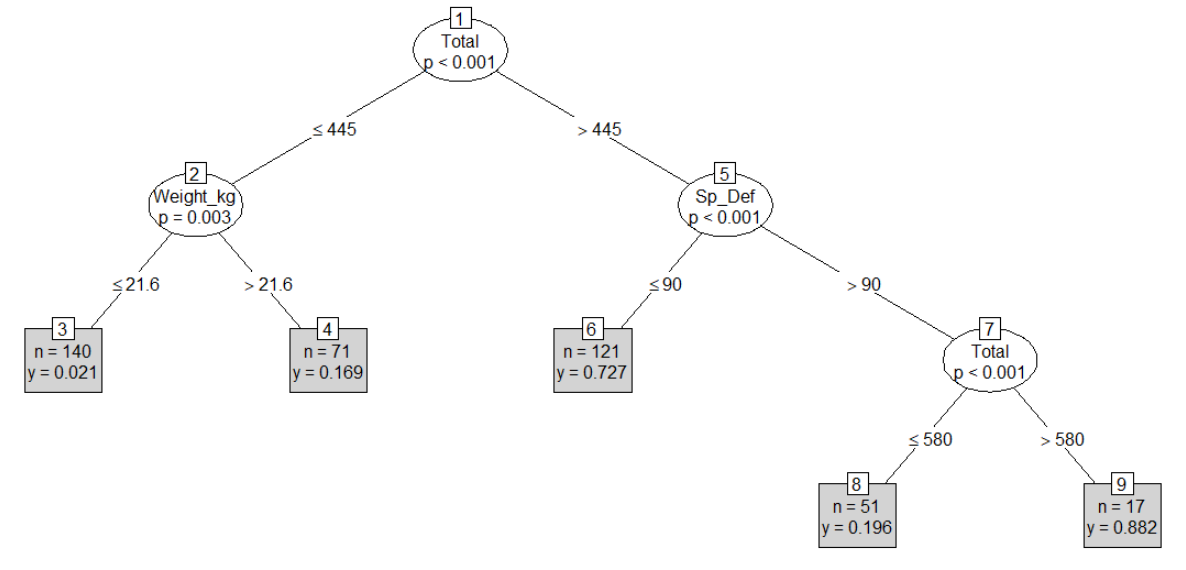
\includegraphics[width=0.98\textwidth]{img/party}
			\end{figure}
		\end{center}
	\end{frame}

	\begin{frame}
		\frametitle{Pacchetto EVTREE}
		\begin{block}{Algoritmo}
			\begin{enumerate}
				\item Inizializzazione casuale (uniforme) popolazione
				\item Valutazione degli individui
				\item Fintantoché la condizione di terminazione non è soddisfatta
				\begin{enumerate}
					\item Selezione dei nodi padri
					\item Applicazione nuovamente la selezione casuale(uniforme)
					\item Valutazione nuovi risultati
					\item Selezione dei sopravvissuti per la nuova generazione
				\end{enumerate}
			\end{enumerate}
		\end{block}
	\end{frame}

	\begin{frame}
		\frametitle{Pacchetto EVTREE}
		\begin{center}
			\begin{figure}
				\lstinputlisting[firstline=225, lastline=227]{code/pokfine.R}
			\end{figure}
			\begin{figure}
				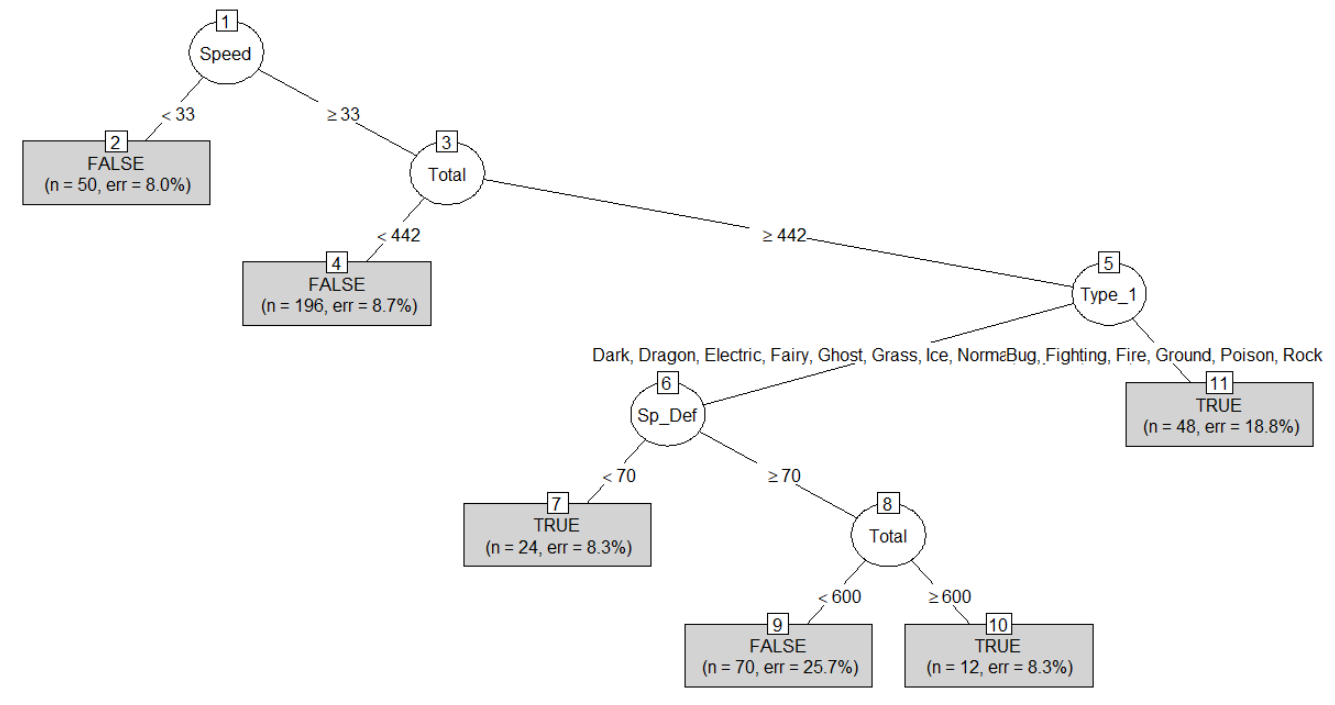
\includegraphics[scale=0.3]{img/evTree}
			\end{figure}
		\end{center}
	\end{frame}

	\begin{frame}
		\frametitle{Confronto pacchetti}
		\begin{center}
			\begin{table}[]
				\resizebox{0.8\textwidth}{!}{\begin{tabular}{ccclccc}
					\cline{1-3} \cline{5-7}
					\multicolumn{3}{|c|}{\textbf{Tree-deviance}}                                                                                                                          & \multicolumn{1}{l|}{} & \multicolumn{3}{c|}{\textbf{Tree-Gini}}                                                                                                                              \\ \cline{1-3} \cline{5-7} 
					\multicolumn{1}{|c}{\cellcolor[HTML]{333333}}                   & \cellcolor[HTML]{C0C0C0}\textbf{FALSE} & \multicolumn{1}{c|}{\cellcolor[HTML]{C0C0C0}\textbf{TRUE}} & \multicolumn{1}{l|}{} & \cellcolor[HTML]{333333}                                       & \cellcolor[HTML]{C0C0C0}\textbf{FALSE} & \multicolumn{1}{c|}{\cellcolor[HTML]{C0C0C0}\textbf{TRUE}} \\ \cline{2-3} \cline{6-7} 
					\multicolumn{1}{|c|}{\cellcolor[HTML]{C0C0C0}\textbf{FALSE}}    & \cellcolor[HTML]{32CB00}175            & \multicolumn{1}{c|}{\cellcolor[HTML]{F56B00}44}            & \multicolumn{1}{l|}{} & \multicolumn{1}{c|}{\cellcolor[HTML]{C0C0C0}\textbf{FALSE}}    & \cellcolor[HTML]{32CB00}154            & \multicolumn{1}{c|}{\cellcolor[HTML]{F56B00}28}            \\
					\multicolumn{1}{|c|}{\cellcolor[HTML]{C0C0C0}\textbf{TRUE}}     & \cellcolor[HTML]{F56B00}23             & \multicolumn{1}{c|}{\cellcolor[HTML]{32CB00}79}            & \multicolumn{1}{l|}{} & \multicolumn{1}{c|}{\cellcolor[HTML]{C0C0C0}\textbf{TRUE}}     & \cellcolor[HTML]{F56B00}44             & \multicolumn{1}{c|}{\cellcolor[HTML]{32CB00}95}            \\
					\multicolumn{1}{|c|}{\cellcolor[HTML]{C0C0C0}\textbf{Accuracy}} & \multicolumn{2}{c|}{\cellcolor[HTML]{34CDF9}79.13\%}                                                & \multicolumn{1}{l|}{} & \multicolumn{1}{c|}{\cellcolor[HTML]{C0C0C0}\textbf{Accuracy}} & \multicolumn{2}{c|}{\cellcolor[HTML]{34CDF9}77.57\%}                                                \\ \cline{1-3} \cline{5-7} 
					\multicolumn{1}{l}{}                                            & \multicolumn{1}{l}{}                   & \multicolumn{1}{l}{}                                       &                       & \multicolumn{1}{l}{}                                           & \multicolumn{1}{l}{}                   & \multicolumn{1}{l}{}                                       \\ \cline{1-3} \cline{5-7} 
					\multicolumn{3}{|c|}{\textbf{Rpart-deviance}}                                                                                                                         & \multicolumn{1}{l|}{} & \multicolumn{3}{c|}{\textbf{Rpart-Gini}}                                                                                                                             \\ \cline{1-3} \cline{5-7} 
					\multicolumn{1}{|c}{\cellcolor[HTML]{333333}}                   & \cellcolor[HTML]{C0C0C0}\textbf{FALSE} & \multicolumn{1}{c|}{\cellcolor[HTML]{C0C0C0}\textbf{TRUE}} & \multicolumn{1}{l|}{} & \cellcolor[HTML]{333333}                                       & \cellcolor[HTML]{C0C0C0}\textbf{FALSE} & \multicolumn{1}{c|}{\cellcolor[HTML]{C0C0C0}\textbf{TRUE}} \\ \cline{1-3} \cline{5-7} 
					\multicolumn{1}{|c|}{\cellcolor[HTML]{C0C0C0}\textbf{FALSE}}    & \cellcolor[HTML]{32CB00}182            & \multicolumn{1}{c|}{\cellcolor[HTML]{F56B00}67}            & \multicolumn{1}{l|}{} & \multicolumn{1}{c|}{\cellcolor[HTML]{C0C0C0}\textbf{FALSE}}    & \cellcolor[HTML]{32CB00}172            & \multicolumn{1}{c|}{\cellcolor[HTML]{F56B00}30}            \\
					\multicolumn{1}{|c|}{\cellcolor[HTML]{C0C0C0}\textbf{TRUE}}     & \cellcolor[HTML]{F56B00}16             & \multicolumn{1}{c|}{\cellcolor[HTML]{32CB00}56}            & \multicolumn{1}{l|}{} & \multicolumn{1}{c|}{\cellcolor[HTML]{C0C0C0}\textbf{TRUE}}     & \cellcolor[HTML]{F56B00}26             & \multicolumn{1}{c|}{\cellcolor[HTML]{32CB00}93}            \\
					\multicolumn{1}{|c|}{\cellcolor[HTML]{C0C0C0}\textbf{Accuracy}} & \multicolumn{2}{c|}{\cellcolor[HTML]{34CDF9}74.14\%}                                                & \multicolumn{1}{l|}{} & \multicolumn{1}{c|}{\cellcolor[HTML]{C0C0C0}\textbf{Accuracy}} & \multicolumn{2}{c|}{\cellcolor[HTML]{34CDF9}82.55\%}                                                \\ \cline{1-3} \cline{5-7} 
					\multicolumn{1}{l}{}                                            & \multicolumn{1}{l}{}                   & \multicolumn{1}{l}{}                                       &                       & \multicolumn{1}{l}{}                                           & \multicolumn{1}{l}{}                   & \multicolumn{1}{l}{}                                       \\ \cline{1-3} \cline{5-7} 
					\multicolumn{3}{|c|}{\textbf{Evtree}}                                                                                                                                 & \multicolumn{1}{c|}{} & \multicolumn{3}{c|}{\textbf{Party}}                                                                                                                                  \\ \cline{1-3} \cline{5-7} 
					\multicolumn{1}{|c|}{\cellcolor[HTML]{333333}}                  & \cellcolor[HTML]{C0C0C0}\textbf{FALSE} & \multicolumn{1}{c|}{\cellcolor[HTML]{C0C0C0}\textbf{TRUE}} & \multicolumn{1}{c|}{} & \multicolumn{1}{c|}{\cellcolor[HTML]{333333}}                  & \cellcolor[HTML]{C0C0C0}\textbf{FALSE} & \multicolumn{1}{l|}{\cellcolor[HTML]{C0C0C0}\textbf{TRUE}} \\
					\multicolumn{1}{|c|}{\cellcolor[HTML]{C0C0C0}\textbf{FALSE}}    & \cellcolor[HTML]{32CB00}166              & \multicolumn{1}{c|}{\cellcolor[HTML]{F56B00}45}             & \multicolumn{1}{c|}{} & \multicolumn{1}{c|}{\cellcolor[HTML]{C0C0C0}\textbf{FALSE}}    & \cellcolor[HTML]{32CB00}177              & \multicolumn{1}{c|}{\cellcolor[HTML]{F56B00}35}             \\
					\multicolumn{1}{|c|}{\cellcolor[HTML]{C0C0C0}\textbf{TRUE}}     & \cellcolor[HTML]{F56B00}32              & \multicolumn{1}{c|}{\cellcolor[HTML]{32CB00}78}             & \multicolumn{1}{c|}{} & \multicolumn{1}{c|}{\cellcolor[HTML]{C0C0C0}\textbf{TRUE}}     & \cellcolor[HTML]{F56B00}21              & \multicolumn{1}{c|}{\cellcolor[HTML]{32CB00}88}             \\
					\multicolumn{1}{|c|}{\cellcolor[HTML]{C0C0C0}\textbf{Accuracy}} & \multicolumn{2}{c|}{\cellcolor[HTML]{68CBD0}76.01\%}                                                      & \multicolumn{1}{c|}{} & \multicolumn{1}{c|}{\cellcolor[HTML]{C0C0C0}\textbf{Accuracy}} & \multicolumn{2}{c|}{\cellcolor[HTML]{68CBD0}82.55\%}                                                      \\ \cline{1-3} \cline{5-7} 
				\end{tabular}}
			\end{table}
		\end{center}
	\end{frame}
